\documentclass[RNAAS]{aastex62}

\newcommand{\vdag}{(v)^\dagger}
\newcommand\aastex{AAS\TeX}
\newcommand\latex{La\TeX}

\submitjournal{RNAAS}

\shorttitle{Non-Detection of Helium for WASP-12b}
\shortauthors{Kreidberg \& Oklop\v{c}i\'{c}}

\begin{document}

\title{Non-Detection of a Helium Exosphere for the Evaporating Hot Jupiter WASP-12b}


\author{Laura Kreidberg}
\affiliation{Harvard-Smithsonian Center for Astrophysics, 60 Garden Street, Cambridge, MA 02138}
\affiliation{Harvard Society of Fellows, 78 Mount Auburn Street, Cambridge, MA 02138}

\author{Antonija Oklop\v{c}i\'{c}}
\affiliation{Harvard-Smithsonian Center for Astrophysics, 60 Garden Street, Cambridge, MA 02138}
A helium exosphere was recently detected around the exoplanet WASP-107b, a
low-density, warm Neptune \citep{spake18}, based on absorption features from the decay
of metastable helium at $10833\,\mathrm{\AA}$ \citep[predicted
by][]{seager00,oklopcic18}. The helium feature provides a new probe of atmospheric escape that is
advantageous in several ways: (1) it is observable with near-infrared facilities
(in contrast to other signposts of atmospheric escape that appear in the
ultraviolet) and (2) it is minimally affected by interstellar absorption, thus opening the door to studying atmospheric escape in a greater number of systems.

Inspired by the WASP-107b detection, we searched archival HST observations of
another evaporating exoplanet, WASP-12b, for signs of a helium exosphere. WASP-12b is a good
candidate for this search: it is one of the hottest known hot
Jupiters \citep[$T_\mathrm{eq} = 2500$ K;][]{hebb09}. At this level of intense irradiation, theory predicts a high rate of escaping atoms and molecules from the planet's atmosphere, and indeed, transit observations in the ultraviolet have revealed a patchy cloud of escaping material \citep{nichols15}.  

For this Note, we reanalyzed three transits observations of WASP-12b from the
Hubble Space Telescope/Wide Field Camera 3 \citep[originally published in][]{kreidberg15b}. These observations used the G102 grism, which spans the
$10833\,\mathrm{\AA}$ helium feature. In our analysis, we used the same methodology as
\cite{kreidberg15b}, except with different spectral binning to include a narrow
band ($70\,\mathrm{\AA}$, the spectrograph's native resolution) centered on the He feature.  
The transmission spectrum (shown in Figure\,\ref{fig:spectrum}) is consistent with that reported in
\cite{kreidberg15b} and shows no evidence for variability between epochs. There
is no significant increase in transit depth at $10833\,\mathrm{\AA}$.  

To estimate the expected absorption signal of WASP-12b at $10833\,\mathrm{\AA}$,
we used the theoretical model described in \cite{oklopcic18}.
In this 1D model, the thermosphere of the planet is assumed to be composed of atomic hydrogen and helium in 9:1 number
ratio. For the thermospheric density and velocity profiles we adopt the
isothermal Parker wind model, assuming the gas temperature of $T=10^4$~K and the
total atmospheric mass loss rate of $4\times 10^{11}$~g~s$^{-1}$ \citep[based on
the results of hydrodynamic simulations of atmospheric escape in WASP-12b
by][]{salz16}. We use the solar irradiance spectrum as the input spectrum. We
consider two cases: one with all the gas included (Model 1), and the other
restricted to gas within the Roche radius (Model 2).

We predict a Model 1 


Under these assumptions, the calculated population of metastable helium within
the Roche radius of the planet produces very little absorption at
$10830\,\mathrm{\AA}$, consistent with the observed non-detection. However, theoretical results are highly dependent on the assumed geometry and parameters of the model, as well as the input stellar spectrum. Although WASP-12 and the Sun are stars of similar spectral types, WASP-12 shows a much lower level of stellar activity (Haswell 2017), and hence its EUV flux, responsible for populating the metastable helium state, might differ considerably from that of the Sun. 

point us to the conclusion that either the gas is dispersed, the star 
is faint at EUV wavelengths, or both. These factors should be
considered in the design of future searches for helium exospheres.

\begin{figure*}[b!]
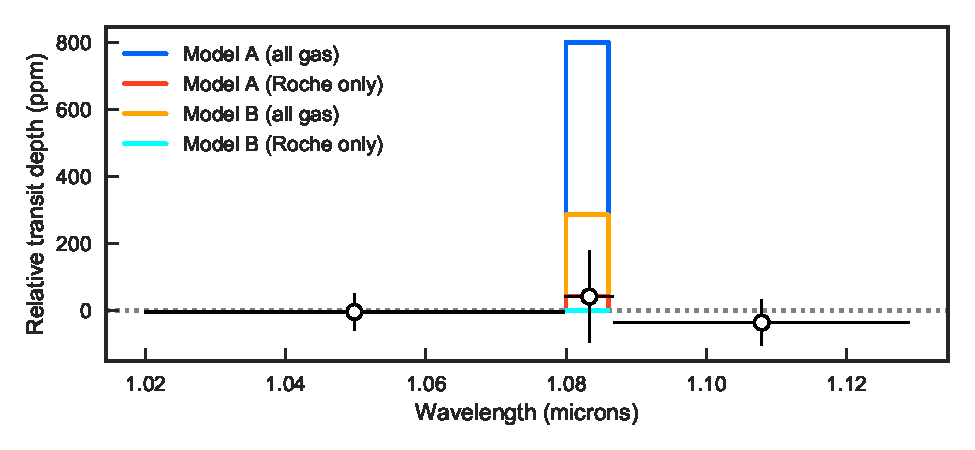
\includegraphics[width = 0.8\textwidth]{Figures/fig1.pdf}
\caption{Transmission spectrum of WASP-12b, compared to model predictions for the strength of the $10833\mathrm{\AA}$ helium line.}
\label{fig:spectrum}
\end{figure*}


\bibliographystyle{aasjournal}
\bibliography{ms.bib}

\end{document}

% End of file `sample62.tex'.
